\documentclass{webofc}
\usepackage{listings}
\usepackage{minted}
\usepackage{subfig}
\usepackage{hyperref}
\usepackage{graphicx}
\usepackage{subcaption}
\usepackage[utf8]{inputenc}
\usepackage{tikz}

\usepackage[varg]{txfonts}

\newminted{cpp}{gobble=2, numbersep=3pt, escapeinside=||, xleftmargin=5mm, framesep=2mm, frame=leftline, baselinestretch=1, fontsize=\scriptsize, linenos=true}
\newmintinline{cpp}{}

\makeatletter
\AtBeginEnvironment{minted}{\dontdofcolorbox}
\def\dontdofcolorbox{\renewcommand\fcolorbox[4][]{##4}}
\makeatother

\usetikzlibrary{shadows, arrows, fit, positioning, matrix, shapes}
\usetikzlibrary{decorations.markings}

% Define colors
\definecolor{my_yellow}{RGB}{255, 253, 217}
\definecolor{my_orange}{RGB}{255, 127, 0}
\definecolor{my_lightblue}{RGB}{105, 186, 249}
\definecolor{my_purple}{RGB}{150, 154, 219}
\definecolor{my_green}{RGB}{90, 194, 160}

% Define block styles  
\tikzset {
  bigbox/.style = {draw, thick, fill=gray!10, rounded corners, rectangle},
  box/.style = {draw, thick, minimum height=0.8cm, minimum width=1.5cm, rounded corners, rectangle, fill=white, anchor=south},
  model/.style = {draw, thick, fill=white, text centered, minimum height=3em, minimum width=4em, rounded corners, drop shadow},
  user/.style = {draw, thick, ellipse, fill=white, text centered, minimum height=3em, minimum width=5em, drop shadow},
  line/.style = {->, thick, color=black, shorten <=2pt, shorten >=2pt, >=stealth'},
  plain/.style = {minimum width=1em},
  %\draw [line, ->] (m1.north) ++(-15pt,-1pt) arc [start angle=-140, end angle=-400, radius=20pt] node[midway] {$T_{M_1}$} ;
  % This works around an issue with node[midway] http://tex.stackexchange.com/questions/38763/how-to-place-a-node-in-the-middle-of-an-arc                
  arcnode/.style 2 args={
    decoration={
                 raise=#1,             
                 markings,   
                 mark=at position 0.5 with {\node[inner sep=0] {#2};}
            },
            postaction={decorate}
    }
}

% Define the layers to draw the diagram
\pgfdeclarelayer{background}
\pgfdeclarelayer{foreground}
\pgfsetlayers{background,main,foreground}

% Draw background
\newcommand{\background}[5]{%
  \begin{pgfonlayer}{background}
    % Left-top corner of the background rectangle
    \path (#1.west |- #2.north)+(-0.5,0.25) node (a1) {};
    % Right-bottom corner of the background rectanle
    \path (#3.east |- #4.south)+(+0.5,-0.25) node (a2) {};
    % Draw the background
    \path[rounded corners, draw=black!50, dashed, name=box]
      (a1) rectangle (a2);
    \path (a1 |- a2) -- (a2) node[midway,below] {\large\textit{#5}};
  \end{pgfonlayer}}

% Define a circled symbol command used throughout the thesis.
\newcommand*\circled[1]{\tikz[baseline=(char.base)]{
            \node[shape=circle,draw,inner sep=2pt] (char) {#1};}}

\begin{document}

\title{Optimizing Frameworks’ Performance Using C++ Modules Aware ROOT}

\author{\firstname{Yuka}
\lastname{Takahashi}\inst{1,2}
\fnsep\thanks{\email{yuka.takahashi@cern.ch}}
        \firstname{Vassil}
        \lastname{Vassilev}\inst{1}\fnsep\thanks
        {\email{vvasilev@cern.ch}}
        \firstname{Oksana}
        \lastname{Shadura}\inst{3}
        \fnsep\thanks{\email{oksana.shadura@cern.ch}} \and
        \firstname{Raphael}
        \lastname{Isemann}\inst{2,4}
        \fnsep\thanks{\email{isemann@student.chalmers.se}}
}

\institute{Princeton University, Princeton, New Jersey 08544, United States
\and
           CERN, Meyrin 1211, Geneve, Switzerland
\and
           University of Nebraska Lincoln, 1400 R St, Lincoln, NE 68588, United States
\and
           Chalmers University of Technology, Chalmersplatsen 4, 41296 Göteborg, Sweden
}

\abstract{%
ROOT is a core HEP framework, broadly used in and outside HEP. Since HEP software frameworks always strive for performance improvements, ROOT was extended with experimental support of runtime C++ Modules. C++ Modules are designed to improve the performance of C++ code parsing. ROOT is parsing and interpreting C++ code during it's runtime, for this case C++ Modules offer a promising way to improve ROOT's runtime performance. This paper presents the results and challenges of integrating C++ Modules into ROOT and its early adoption to CMSSW software stack.
}
%
\maketitle
%
\section{Introduction}
\label{intro}

The core part of ROOT is the C++ interpreter \textttt{Cling}, which is build on the top of the C++ compiler Clang. The interpreter allows users to have interactive ROOT sessions. It also serves as a backend for ROOT's language bindings such as ROOT Python extension module PyROOT.

To offer these features, Cling has to parse source code during runtime. This includes not only the code manually entered by the user from a command line, but also a multitude of the header files coming from libraries and frameworks. The header file parsing can negatively affect ROOT's performance as it consumes notable amounts of memory and CPU time.

Since the inefficient header parsing in C++ is a well-known issue, the C++ standard introduced C++ Modules, delivering a compact, efficient representation of header files. Modules are becoming a promising technology for C++ community and since the adoption of C++ Modules into ROOT was already proposed earlier in paper \cite{vassil-paper} and we implemented them in ROOT and its interpreter Cling. This allowed us to avoid the expensive parsing of headers and improve ROOT's runtime performance.

\section{Background}
\label{background}

Even before C++ Modules, ROOT has been heavily optimized and employs several mechanisms to improve the performance of the interpreter. In this section we will discuss three of the existing mechanisms in the context of C++ Modules: The ROOT precompiled header (PCH); ROOTMAP files (ROOTMAP) and RDICT files.

\subsection{Optimizing ROOT using a PCH}
\label{pch}
ROOT ships with a precompiled header containing a subset of ROOT's components. This precompiled header reduces the CPU and memory cost for ROOT’s heavily used libraries. The precompiled header technology has been well-understood for decades. It is an efficient on-disk representation of the state of the compiler after parsing a set of headers. It can be loaded before starting the next instance to avoid doing redundant work. However, this approach limits compiler to use only a single PCH, as it's usually too involved to merge multiple compiler states loaded from different PCH files. ROOT’s dictionary generator, \textit{rootcling}, generates one PCH file at build time. This PCH file is loaded on startup and ROOT proceeds to lazily evaluate the code from the file when needed.

The PCH is by design monolithic and not extensible. This is a problem for third party libraries who want to improve the performance of their code with a PCH. They cannot provide a second PCH file with their code as this is not possible by design. For ROOT developers the PCH brings the problem that changing a single header requires the regeneration of the whole PCH file.

A less restrictive alternative to PCH files is C++ Modules (PCM files). Unlike a PCH, PCM files are designed to be separable, so that multiple PCMs can be attached to the same interpreter or compiler simultaneously. This means that it is possible to split up the content of a single PCH into multiple PCMs as shown in Figure \ref{fig:pchandPCM}. Also, it is possible to rebuild only a subset of all attached PCMs. In ROOT, a single PCM file usually corresponds to a single library.

The implementation of C++ Modules in ROOT is based on Clang's implementation, which is called as an API from ROOT. Clang uses configuration files called Module Maps for defining the contents of a C++ Module. To stay consistent with Clang, ROOT also uses Module Map files to configure Module contents.

\begin{figure}[!h]
  \centering
  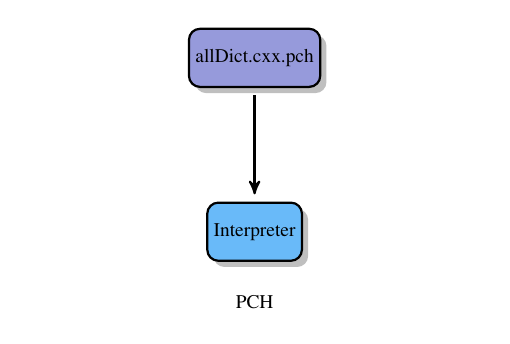
\begin{tikzpicture}[outer sep=0.05cm, node distance=0.8cm, scale=0.7, transform shape]
        
    \node[model, fill=my_purple, name=pch] (pch) {allDict.cxx.pch};
    \node[model, fill=my_lightblue, name=interpreter, below=2cm of pch] (interpreter) {Interpreter};

    \draw[line, ->] (pch.south) -- (interpreter);
    
    \node [below=1cm, align=flush center,text width=8cm] at (interpreter) { PCH };
  \end{tikzpicture}
  \hfill
  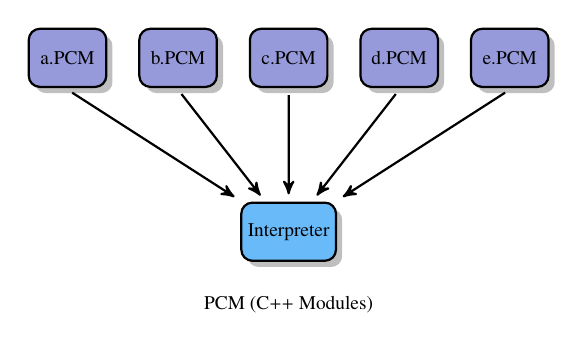
\begin{tikzpicture}[outer sep=0.05cm, node distance=0.8cm, scale=0.7, transform shape]
        
    \node[model, fill=my_purple, name=a] (a) {a.PCM};
    \node[model, fill=my_purple, name=b, right=0.5cm of a] (b) {b.PCM};
    \node[model, fill=my_purple, name=c, right=0.5cm of b] (c) {c.PCM};
    \node[model, fill=my_purple, name=d, right=0.5cm of c] (d) {d.PCM};
    \node[model, fill=my_purple, name=e, right=0.5cm of d] (e) {e.PCM};

    \node[model, fill=my_lightblue, name=interpreter, below=2cm of c] (interpreter) {Interpreter};

    \draw[line, ->] (a.south) -- (interpreter);
    \draw[line, ->] (b.south) -- (interpreter);
    \draw[line, ->] (c.south) -- (interpreter);
    \draw[line, ->] (d.south) -- (interpreter);
    \draw[line, ->] (e.south) -- (interpreter);
    
    \node [below=1cm, align=flush center,text width=8cm] at (interpreter) { PCM (C++ Modules) };

  \end{tikzpicture}
  \caption{Comparison of PCH and C++ Modules in ROOT. The content of a single PCH can be separated to multiple PCMs, which makes PCMs modular.}
  \label{fig:pchandPCM}
\end{figure}

\subsection{Optimizing third-party code with ROOTMAP and RDICT}
\label{dictgen}

ROOTMAP files are used by ROOT to map unknown symbols and identifiers to libraries. When encountering an unknown symbol or identifier, ROOT uses ROOTMAP files to load the corresponding library. An advantage of this approach is that ROOTMAP files allow ROOT to only parse headers of libraries that are actually used. The expensive header parsing only happens when it is necessary.

RDICT files efficiently store information needed for serialization and deserialization of data types. They allow ROOT to perform IO operations on these data types without loading the respective code from the PCH or parsing the respective library headers.

\begin{listing}[h]
    \noindent
    \begin{minipage}[h]{\textwidth}
    \begin{cppcode*}{}
// Foo.h
    |\label{line:foobar}|namespace foo { struct bar{}; }
    |\label{line:structs}|struct S{};

// libFoo.rootmap
    |\label{line:decls}|{ decls }
    namespace foo { }
    struct S;
 
    |\label{line:libfoo}|[ libFoo.so ]
    # List of selected classes
    class bar
    struct S

// G__Foo.cxx (aka libFoo dictionary)
    namespace {
      void TriggerDictionaryInitialization_libFoo_Impl() {
        static const char* headers[] = {"Foo.h"}
        // More scaffolding
        extern int __Cling_Autoloading_Map;
        namespace foo{struct __attribute__((annotate("$ClingAutoload$Foo.h"))) bar;}
        struct __attribute__((annotate("$ClingAutoload$Foo.h"))) S;
       // More initialization scaffolding.
    }
    \end{cppcode*}
    \end{minipage}
    \caption{The example of ROOT dictionary for {\it libFoo}. {\it Foo.h} is the header file which contains the definition. {\it libFoo.rootmap} is generated by rootcling, and it contains the forward declaration of {\it Foo.h}. {\it G\_\_Foo.cxx} is injected in the {\it libFoo} object file, and is called when {\it libFoo} is being loaded to ROOT.}
    \label{list:foo}
\end{listing}

At startup, ROOT will locate all files with extension {\it *.rootmap}. It parses the code in Listing \ref{list:foo} Line \ref{line:decls} \{decls\} section and creates an internal map for the entities defined in Listing \ref{list:foo} Line \ref{line:libfoo} [libFoo.so] section. Upon seeing an unknown identifier, the implementation searches in the database if this is a known entity.

\begin{listing}[h]
    \noindent
    \begin{minipage}[h]{\textwidth}
    \begin{cppcode*}{linenos=true}
    |\label{line:prompt1}|root [] S *s;           // Does not require a definition.
    |\label{line:prompt2}|root [] foo::bar *baz1; // Does not require a definition.
    |\label{line:prompt3}|root [] foo::bar baz2;  // Requires a definition.
    \end{cppcode*}
    \end{minipage}
    \caption{Illustrative example for usage of the ROOT dictionary contents.}
    \label{list:prompt}
\end{listing}

Listing \ref{list:prompt} shows the efforts which ROOT does to avoid parsing redundant code. {\it S} is defined in Line \ref{line:structs} in Listing \ref{list:foo} and {\it foo::bar} is defined in Line \ref{line:foobar} in Listing \ref{list:foo}. Listing \ref{list:prompt} Line \ref{line:prompt1} does not require a definition and the forward declaration consumed at the initialization time is sufficient, so the parsing of {\it Foo.h} is not required. The behavior of Line \ref{line:prompt1} in Listing \ref{list:prompt} is equivalent to Lines \ref{line:line2beggining} and \ref{line:rootss} in Listing \ref{list:line2}.

\begin{listing}[h]
    \noindent
    \begin{minipage}[h]{.7\textwidth}
    \begin{cppcode*}{}
    |\label{line:line2beggining}|root [] namespace foo { }; struct S;
    |\label{line:rootss}|root [] S *s; // Implicitly at ROOT startup
    root [] foo::bar /*store parsing state*/
    gSystem->Load("Foo");
    // More scaffolding.
    extern int __Cling_Autoloading_Map;
    namespace foo{struct __attribute__((annotate("$ClingAutoload$Foo.h"))) bar;}
    struct __attribute__((annotate("$ClingAutoload$Foo.h"))) S;
    // More initialization scaffolding.
    |\label{line:beforerestoreparsing}|/*restore parsing state*/ *baz1;
    
    |\label{line:restoreparsing}|#include <Foo.h>/*restore parsing state*/;
    \end{cppcode*}
    \end{minipage}
    \caption{Information flow from {\it libFoo} dictionary.}
    \label{list:line2}
\end{listing}

Line \ref{line:prompt2} in Listing \ref{list:prompt} also does not require a definition. The second identifier lookup fails, but ROOT knows that {\it foo::bar} is in {\it libFoo} by the information from ROOTMAP files in Listing \ref{list:foo} Line \ref{line:libfoo}. It dlopens {\it libFoo} which in turn, during its static initialization, inserts annotated forward declaration as shown in {\it G\_\_Foo.cxx}. This resolves {\it foo::bar} which avoids the parsing of {\it Foo.h} at relatively small overhead. The loading of the annotated forward declarations can happen at any time during parsing. This so-called "recursive parsing" is a code path that exists only in ROOT, and is not exercised by Clang itself. The behavior of Line \ref{line:prompt2} is equivalent to Listing \ref{list:line2} Lines \ref{line:line2beggining} to \ref{line:beforerestoreparsing}.

Line \ref{line:prompt3} in Listing \ref{list:prompt} requires a definition and the implementation behaves exactly as in Line \ref{line:prompt2}. When a definition is required, it reads the information in the annotation and also parses {\it Foo.h} as is shown in Line \ref{line:restoreparsing} in Listing \ref{list:line2}. The Line \ref{line:prompt3} in Listing \ref{list:prompt} behavior is equivalent to Line \ref{line:line2beggining} to \ref{line:restoreparsing} in Listing \ref{list:line2}.

ROOTMAP files and RDICT files are important for ROOT's performance. However, they require various mechanisms to work together and can fail in corner cases. Also, due to the complicated way they are implemented on top of the Clang API, they have a high probability to become unusable if certain parts of Clang's internal behavior changes. C++ Modules can partly replace their performance benefits while also offering a more stable implementation.

\section{Implementation}
\label{implementation}

An implementation of the C++ Modules concept itself exists in the LLVM frontend Clang \cite{clang-Modules-doc} which works as an API for ROOT and is included in ROOT source tree. It is possible to compile ROOT with C++ Modules with other C++ compilers such as GCC, as it also compiles Clang in the source and ROOT calls its API. Clang supports the Modules TS and hosts Modules research and development work. Clang's implementation encourages incremental, bottom-up adoption of the C++ Modules \cite{Smith-cppcon}. The implementation is designed to work for C, C++, ObjectiveC, ObjectiveC++ and Swift \cite{Moduralize-doc}. Users can enable the Modules feature without modifications in header files. Clang allows users to specify Module interfaces in a dedicated file, called a Module Maps file. A Module Map file expresses the mapping between a Module file and a collection of header files. It can be mounted using the compiler’s virtual file system overlay mechanism to non-writable library installation paths. In practice, a non-invasive modularization can be done easily by introducing a Module Map file. In some cases the Module Map files can be automatically generated if the build system knows about the list of header files in every package.

Several steps were taken to adopt C++ Modules in ROOT. First, we supported compiling ROOT with C++ Modules, which halfed ROOT's build time. This effort includes generating Module Map files and resolving cyclic header dependency inside ROOT. Next, we taught rootcling dictionary generator to generate PCM files attached with I/O information. We taught ROOT to preload all PCMS at the startup time in order to make declaration available without \#including the appropriate headers. Also, we implemented the autoloading of libraries in ROOT which does not depend on old infrastructure (ROOTMAPS), which gives correctness benefits demonstrated in section \ref{correctness} and is more efficient compared to ROOTMAPS.

%TODO: REWORD: This is because we can infer the library name from the PCM name. Beyond that, we have done a large amount of performance optimization in ROOT and Clang.

For the C++ Modules adoption in experiments, we have been working closely with CMSSW team \cite{cms}. ROOT can already be compiled with runtime C++ in CMS environment, and we will enable PCM generation for their libraries one by one. We can gradually migrate dictionary generation to PCM, as our current implementation falls back to ROOTMAP when a PCM is not generated. It enables us to incrementally migrate from the old to the new infrastructure.

\subsection{Registration Mechanism and Automatic Discovery of C++ declarations}
\label{subsec:preloading}

\begin{listing}[h]
    \noindent
    \begin{minipage}[h]{.7\textwidth}
    \begin{cppcode*}{}
    |\label{line:importroot}|root [] import ROOT.*;
    |\label{line:importfoo}|root [] import Foo.*;
    root [] foo::bar *baz1;
    \end{cppcode*}
    \end{minipage}
    \caption{Pseudocode shows the loading of all Modules at the ROOT startup time.}
    \label{list:implicit-include}
\end{listing}

A C++ Modules aware ROOT preloads all Modules at its startup time. Listing \ref{list:prompt} becomes equivalent to Listing \ref{list:implicit-include}. Listing \ref{list:implicit-include} shows the example of implicit \#include, where {\it foo::bar} can be used without even including {\it Foo.h}. With Modules, this feature is supported by importing all Modules at the startup time, as shown in Line \ref{line:importroot} and \ref{line:importfoo}. Currently, importing all Modules comes with a constant performance overhead which we explain in detail in section \ref{performance}.

However, there is another way to support this feature: the Global Modules Index, which makes the list of identifiers and PCMs at the initialization time. Upon the identifier lookup failure, the interpreter can refer to the list to decide which PCM to load. The possible drawback of this implementation is that the interpreter has no control over where the lookup failure can happen. It can happen inside a nested scope where importing a PCM may cause an incomprehensible error.

Regarding automatic discovery of C++ declarations, a naive implementation of this feature would require the inclusion of all reachable library descriptors at ROOT startup time, which is not feasible. ROOT inserts a set of optimizations from ROOTMAP files to fence itself from the costly full header inclusion. Unfortunately, several of them are home-grown and in a few cases inaccurate causing a notable technical debt.

With runtime C++ Modules, ROOT iterates through libraries found in Prebuilt Modules Paths and LD\_LIBRARY\_PATH until it finds the definition of the currently sought mangled name. It searches the library in Prebuilt Modules Path first as it is more likely that the symbols are in ROOT related library. When it fails, the implementation fall-backs to searching libraries from LD\_LIBRARY\_PATH for system library auto-loading. The overhead is remarkably low as it is only looking into a 64-byte hash in the library to determine whether this library likely has a definition or not, which is called bloom filter. Not only the symbols defined in regular symbol tables but also the dynamic symbols can be autoloaded as we are also checking .dynsym section where the dynamic symbols are defined. This feature is new and is not supported without C++ Modules in ROOT. The benefit of this implementation can be seen in Section \ref{correctness}.

\section{Results}
\label{results}

\subsection{Performance Results}
\label{performance}

\begin{figure}
\centering
    \begin{minipage}{.48\textwidth}
    \subfloat[] {\label{fig:perfBuildingROOT:a} 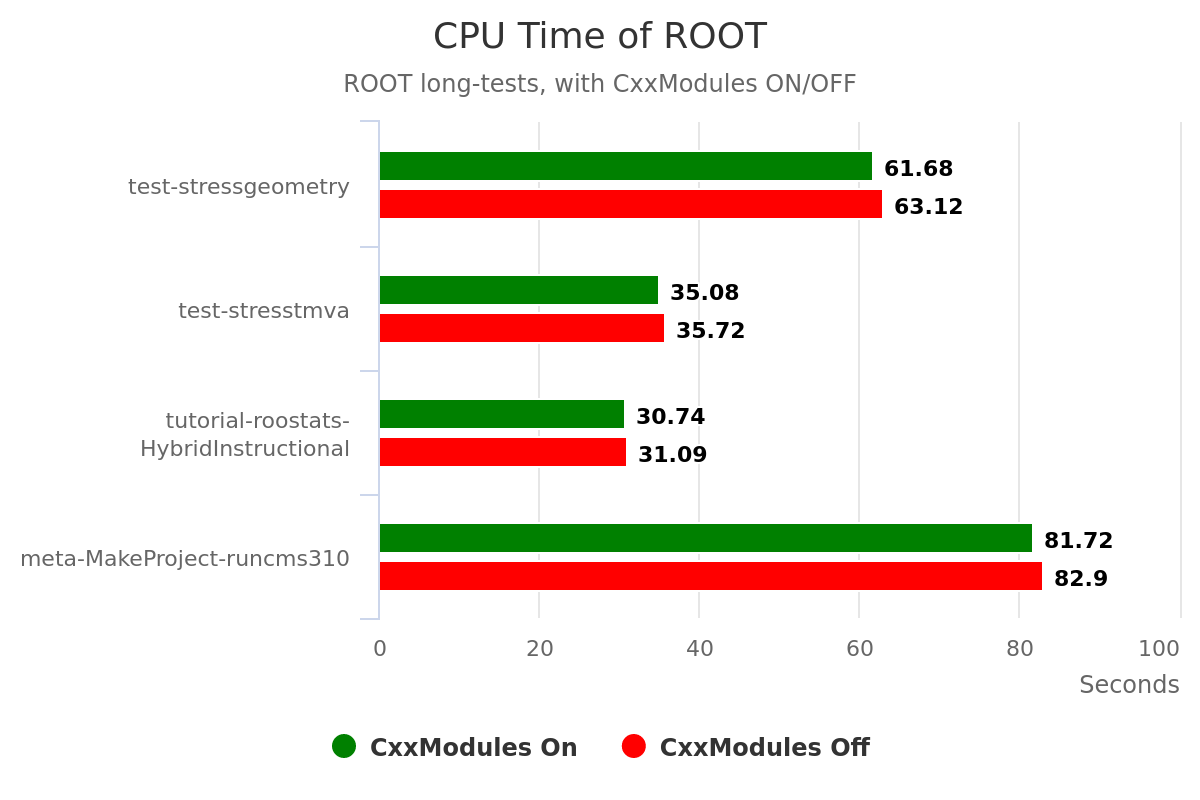
\includegraphics[width=\textwidth]{Long_CPU.png}}
   \end{minipage}\hfill
    \begin{minipage}{.48\textwidth}
    \subfloat[] {\label{fig:perfBuildingROOT:a} 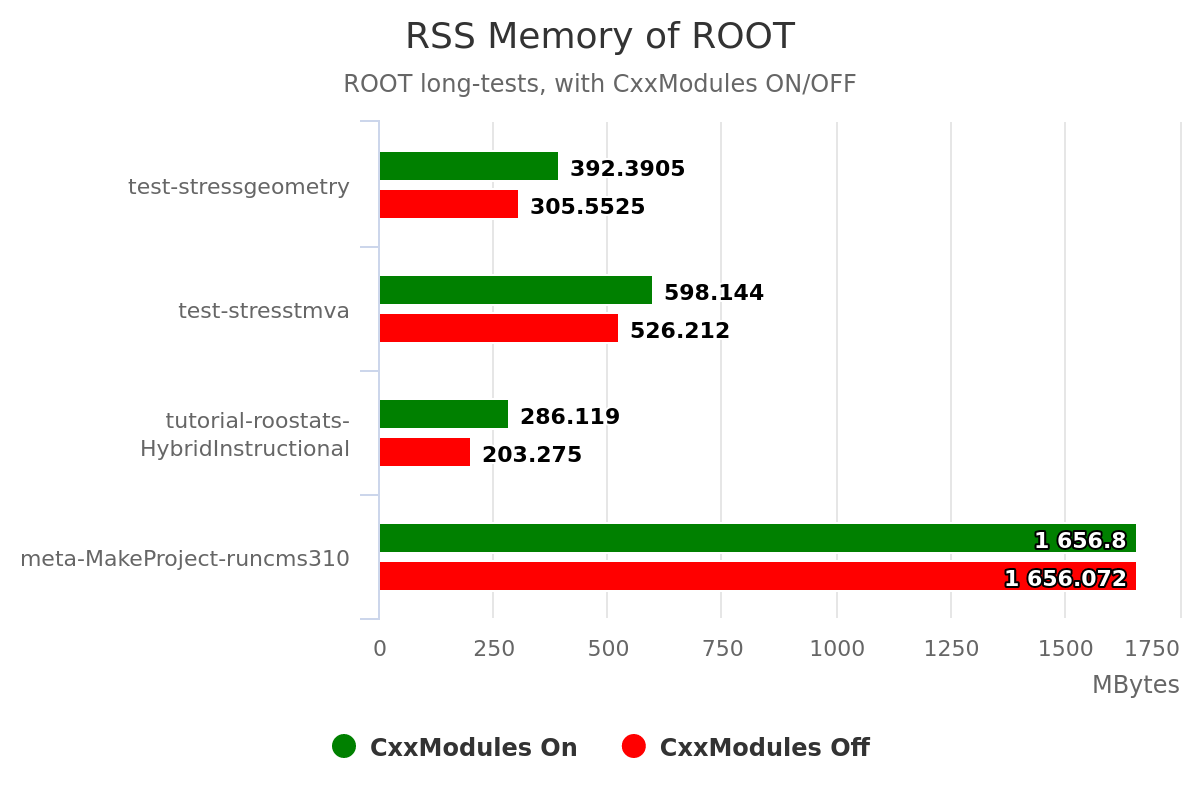
\includegraphics[width=\textwidth]{Long_RSS.png}}
   \end{minipage}
   
    \begin{minipage}{.48\textwidth}
    \subfloat[] {\label{fig:perfBuildingROOT:a} 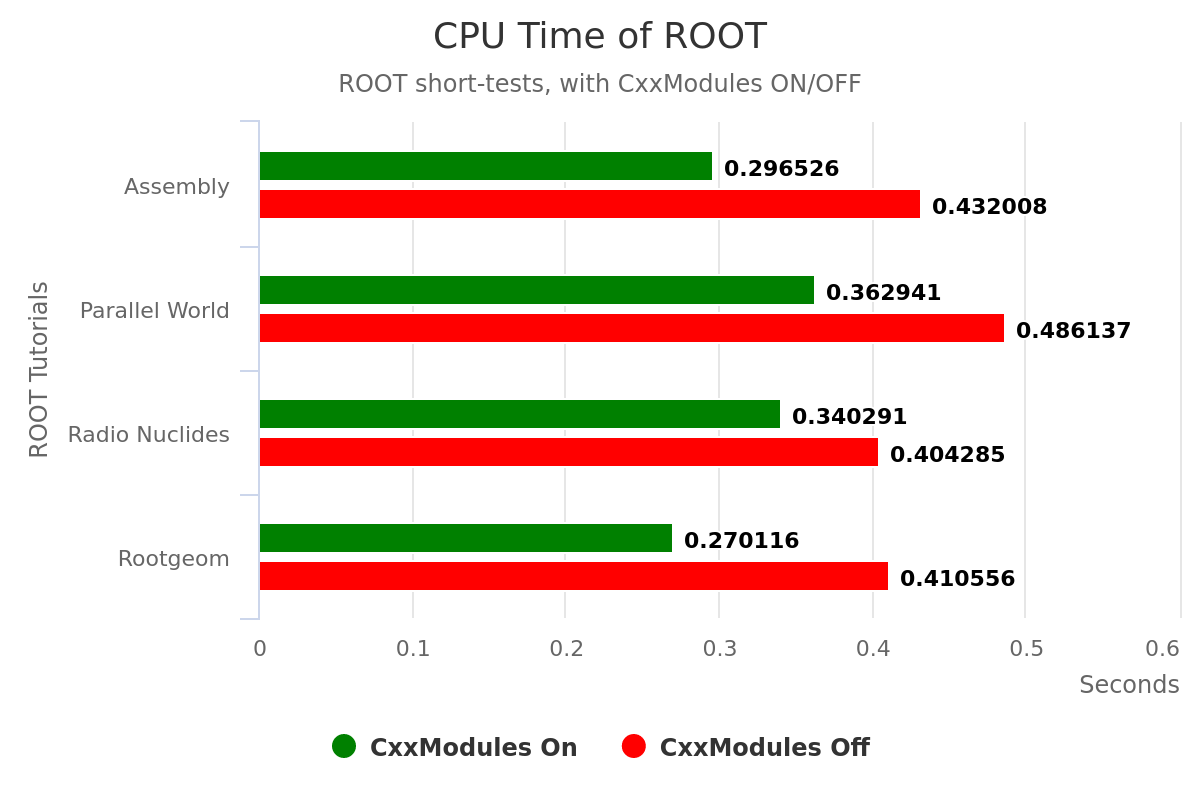
\includegraphics[width=\textwidth]{Short_CPU.png}}
   \end{minipage}\hfill
    \begin{minipage}{.48\textwidth}
    \subfloat[] {\label{fig:perfBuildingROOT:a} 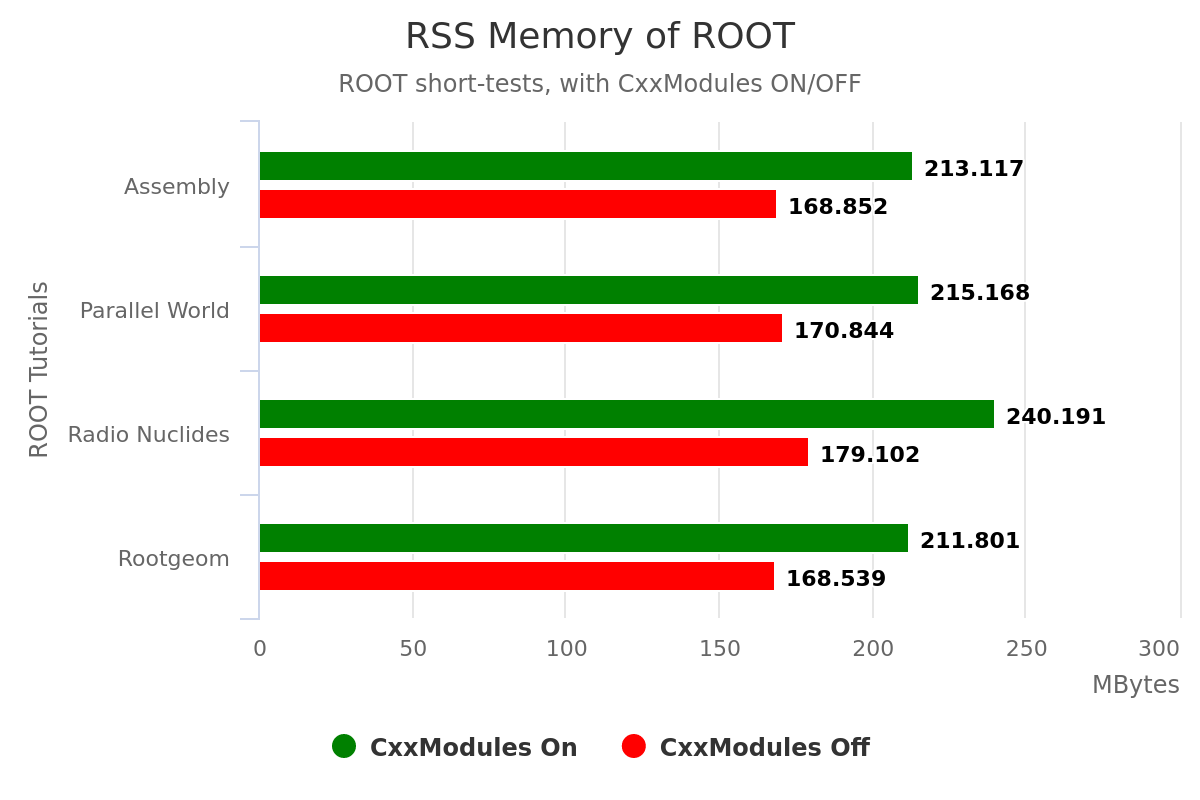
\includegraphics[width=\textwidth]{Short_RSS.png}}
   \end{minipage}
\caption{Performance results: (a) and (c) are the measurement of CPU Time. (b) and (d) are the measurement of RSS. (a) and (b) are measuring long tests (over 30 seconds) in ROOT with and without runtime C++ Modules. (c) and (d) are measuring short tests which is not in PCH.}
\label{fig:performance1}
\end{figure}

\begin{figure}
\centering
    \begin{minipage}{.48\textwidth}
    \subfloat[] {\label{fig:perfBuildingROOT:a} 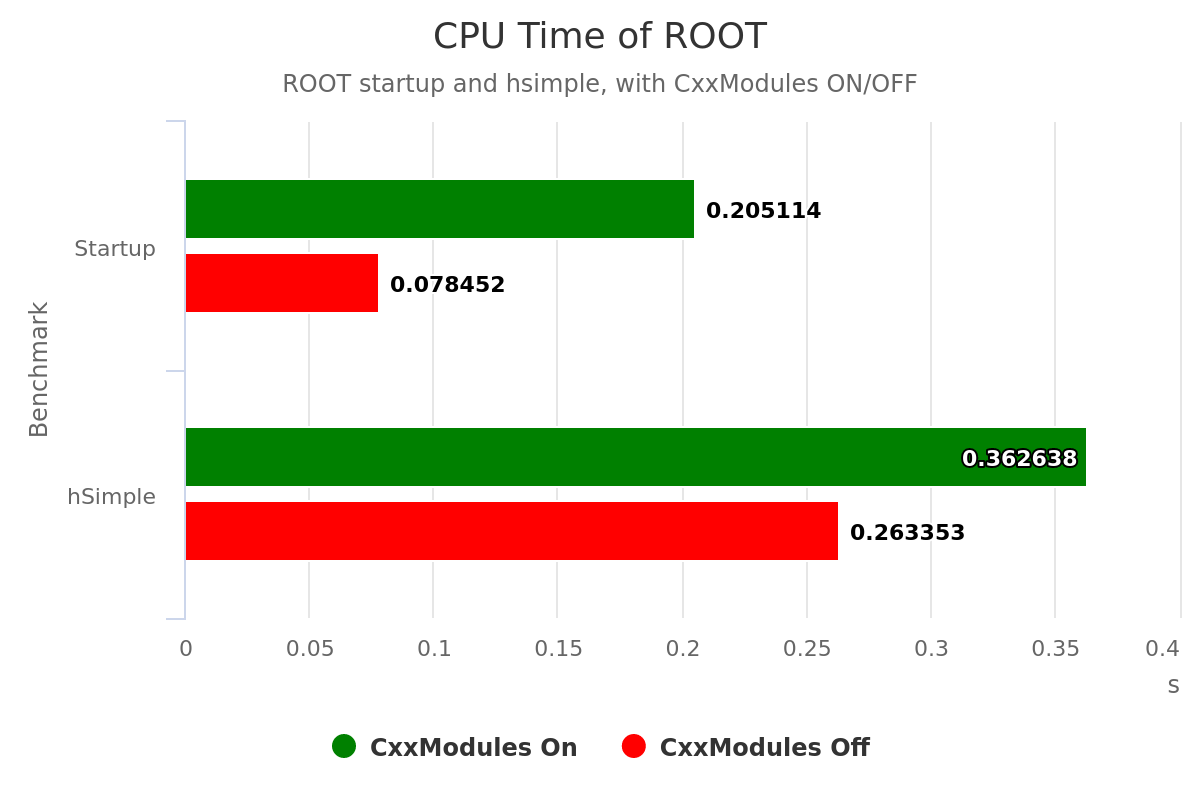
\includegraphics[width=\textwidth]{Startup_CPU.png}}
   \end{minipage}\hfill
    \begin{minipage}{.48\textwidth}
    \subfloat[] {\label{fig:perfBuildingROOT:a} 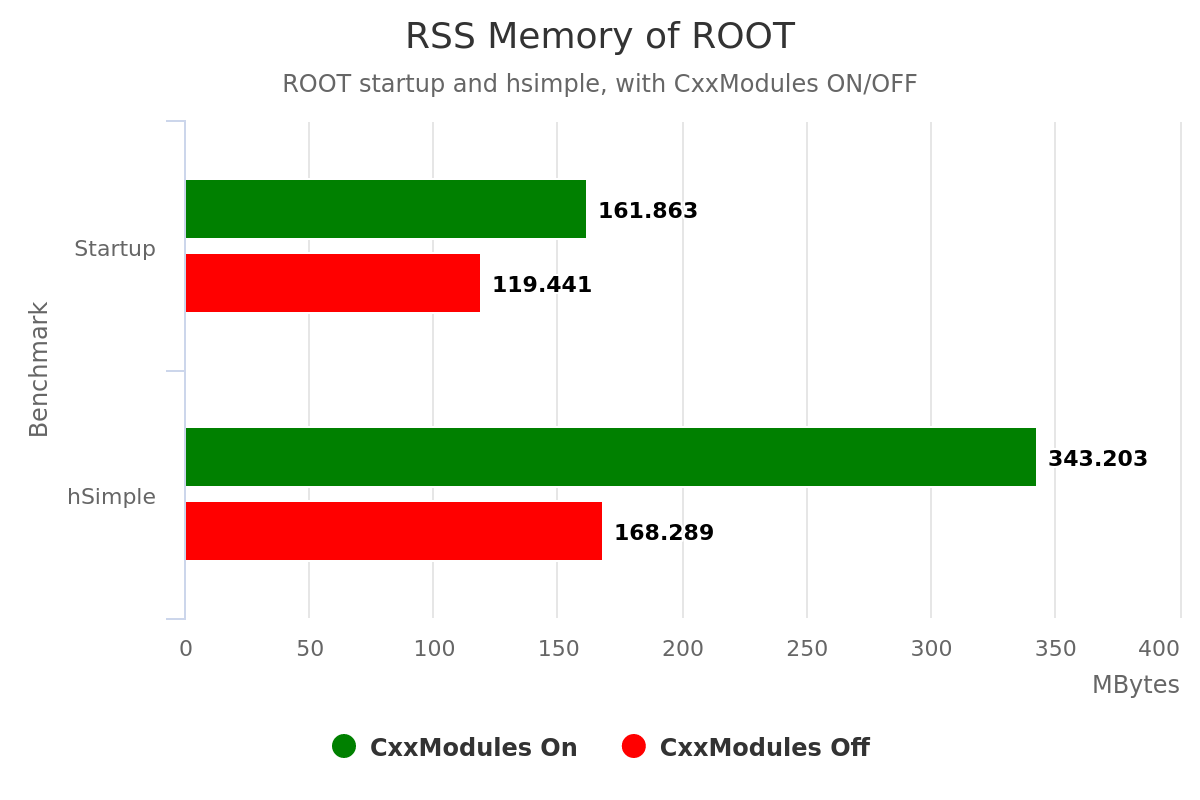
\includegraphics[width=\textwidth]{Startup_RSS.png}}
   \end{minipage}
\caption{Basic benchmarks: The start-up initialization of ROOT and hSimple tutorial.} 
\label{fig:performance2}
\end{figure}

Performance measurements in ROOT are often done by running tutorials and tests in ROOT.
We measured the performance with {\it Archlinux 4.18.16 GNU/Linux, Intel(R) Core(TM) i7-8550U CPU} and {\it Ubuntu 18.04.1 LTS, i7-7500U NVIDIA GeForce 940MX}.
Figure \ref{fig:performance1} and Figure \ref{fig:performance2} are the performance results we receive from Modules compared to PCH and Textual Headers, which are similar to the workloads of the experiment software stacks.

The CPU time of ROOT is measured in (a) and (c) in Figure \ref{fig:performance1} and (a) in Figure \ref{fig:performance2}, whereas (b) and (d) in Figure \ref{fig:performance1} and (b) in Figure \ref{fig:performance2} are measuring the residential memory of ROOT.

ROOT long tests are the tests which take more than 30 seconds, and are measured in (a) and (b) in Figure \ref{fig:performance1}. (c) and (d) in Figure \ref{fig:performance2} are testing short tests which are not in PCH, which means that they are still using textual includes. Thus from those tests, we can get a rough assumption of the performance result we will get from modularizing experiments. Figure \ref{fig:performance2} is measuring the startup of ROOT and executing the hsimple tutorial, to show the actual startup time overhead we have from preloading PCMs.

The RSS memory regression which can be seen in Figure \ref{fig:performance1} (d) and in Figure \ref{fig:performance2} (b) are mostly due to importing all C++ Modules at the startup. The RSS overhead increases in proportion to the number of the preloaded Modules. The startup memory overhead is between 40-60 MB depending on the concrete configuration. However, when the workload increases (Figure \ref{fig:performance1} (b)) we notice that the overall memory performance decreases in the number of cases.

The CPU time regression in Figure \ref{fig:performance2} (a) and in Figure \ref{fig:performance1} (c) are also due to importing all PCMs at the startup time. However, in Figure \ref{fig:performance1} (a) the performance of C++ Modules is better than PCH by 1 or 2 seconds. It shows that C++ Modules can perform better when the workload of the users' code increases.

The performance of the technology preview is dependent on many factors such as the configuration of ROOT and a workflow. We also implemented a continuous performance monitoring tool \cite{rootbench} where we compare the performance of the technology preview with respect to ROOT without C++ Modules.

\subsection{Correctness and Extra usability features}
\label{correctness}

\begin{listing}[h]
    \noindent
    \begin{minipage}[h]{.48\textwidth}
    \begin{cppcode*}{}
root [] gMinuit // Cannot load variable
IncrementalExecutor::executeFunction:
symbol 'gMinuit' unresolved while
linking [Cling interface function]!
    \end{cppcode*}
    \end{minipage}\hfill
    \begin{minipage}[h]{.48\textwidth}
    \begin{cppcode*}{}
root [] gMinuit // Could load libMinuit
(TMinuit *) nullptr
    \end{cppcode*}
    \end{minipage}
    \caption{Correctness results: The left-hand side is ROOT without runtime C++ Modules, which cannot autoload extern global variables such as gMinuit. The right-hand side is ROOT with runtime C++ Modules, with which gMinuit can be autoloaded.}
    \label{list:gMinuit}
\end{listing}

\begin{listing}[h]
    \noindent
    \begin{minipage}[h]{.48\textwidth}
    \begin{cppcode*}{}
root [] #include <m17n-core.h> // System header
root [] m17n_init_core()
IncrementalExecutor::executeFunction:
symbol 'm17n_init_core' unresolved while
linking [Cling interface function]!
    \end{cppcode*}
    \end{minipage}\hfill
    \begin{minipage}[h]{.48\textwidth}
    \begin{cppcode*}{}
root [] #include <m17n-core.h>
root [] m17n_init_core()
root [] // Autoload system library
    \end{cppcode*}
    \end{minipage}
    \caption{Autoloading of system libraries: Left-hand side is ROOT without runtime C++ Modules, which cannot autoload a system library. Right-hand side is ROOT with runtime C++ Modules, where ROOT can autoload the corresponding system library.}
    \label{list:system}
\end{listing}

As shown in Listing \ref{list:gMinuit}, gMinuit is an extern variable which cannot be autoloaded by ROOT without Modules as the forward declaration is not declared in ROOTMAP files. However, with Modules, we can automatically resolve symbols and cases like those are correctly handled. Moreover, Listing \ref{list:system} shows that ROOT can also autoload system libraries with dynamic symbols. Module's autoloading implementation iterate through LD\_LIBRARY\_PATH which also includes system libraries. The implementation details are thoroughly discussed in Section \ref{implementation}.

\section{Limitations and Future work}
\label{limitationsandfuture}

Even though ROOT now supports C++ Modules, there remain some problems that need to be solved before C++ Modules are fully usable for developers and users. One limitation is that Clang does not explicitly support the relocation of implicitly-built PCM files. It is possible to patch Clang to work with implicitly-built PCM, but it is better to have an official support. The limitation comes from the fact that Modules files store paths of the configuration and source files in them. These paths will become invalid once the build directory has been moved.

%% TODO: FIXME and reenable? Another issue is that the automatic import of code into user code can introduce namespace pollution. Although this is a useful prompt feature from which ROOT's users can benefit from, it requires a lookup in the table which give a constant overhead. Also, the user can end up not noticing their mistakes in code as ROOT can automatically \#include appropriate header files, which users might not intended. %English broken

One significant issue is that C++ Modules are currently not as efficient as ROOT's PCH when used in a minimal environment without experiment frameworks. In this situation the PCH is a more efficient as it was optimized for the specific setup of ROOT. ROOT's C++ Modules however are kept back by two issues. One issue is the additional overhead coming from management data structures that make PCMs more extensible than the PCH. The other issue is that C++ Modules in ROOT are currently not as optimized as the PCH. Especially the preloading of Modules on startup needs to be optimized as explained in section \ref{implementation}.

Our ultimate goal is to make this feature a default in ROOT. In order to archieve this, we will give support to experiments such as CMSSW and will continue optimizing the performance.

\section{Acknowledgments}

This work has been supported by an Intel Parallel Computing Center grant, by U.S. National Science Foundation grants PHY-1450377, OAC-1450377 and PHY-1624356, and by the U.S. Department of Energy, Office of Science.

The authors would like to thank CERN/EP-SFT and the ROOT team in particular.

\begin{thebibliography}{plain}

\bibitem{vassil-paper}
Vassil Vassilev, J. Phys.: Conf. Ser. \textbf{898}, 072023 (2017)

\bibitem{clang-Modules-doc}
Clang Modules Documentation, \url{http://clang.llvm.org/docs/Modules.html}, accessed: 2018-24-11

\bibitem{Moduralize-doc}
Modularize Documentation, \url{http://clang.llvm.org/extra/modularize.html}, accessed: 2018-24-11

\bibitem{Gregor-cppcon}
Doug Gregor, cppCon 2016, Modules, URL \url{http://llvm.org/devmtg/2012-11/#talk6}

\bibitem{Klimek-cppcon}
Manuel Klimek, cppCon 2016, Deploying C++ Modules to 100s of Millions of Lines of Code, URL \url{https://cppcon2016.sched.com/event/7nM2/deploying-c-Modules-to-100s-of-millions-of-lines-of-code}

\bibitem{Smith-cppcon}
Richard Smith, cppCon 2016, There and Back Again: An Incremental C++ Modules Design, URL \url{https://cppcon2016.sched.com/event/7nM6/there-and-back-again-an-incremental-c-Modules-design}

\bibitem{David-talk}
David Blaikie, LLVM developer's meeting 2018, Build Impact of Explicit and C++ Standard Modules, URL \url{https://youtu.be/b-iiA18BRCQ}

\bibitem{rootbench}
Oksana Shadura, CHEP 2018 preprint, Continuous Performance Benchmarking Framework for ROOT

\bibitem{cms}
CMS Collaboration, “The CMS experiment at the CERN LHC”, JINST 3 (2008) S08004. doi:10.1088/1748-0221/3/08/S08004.

\end{thebibliography}

\end{document}


% Notes

<div id='footer'><table width='100%'><tr><td class='right'><a href='http://fusioninventory.org/'><span class='copyright'>FusionInventory 9.1+1.0 | copyleft <img src='/glpi/plugins/fusioninventory/pics/copyleft.png'/>  2010-2016 by FusionInventory Team</span></a></td></tr></table></div>

